\documentclass[14pt,final,titlepage,pscyr]{hedsemwork}
\usepackage[russian]{babel}
\usepackage[utf8]{inputenc}
\usepackage[derivative]{hedmaths}
\usepackage{graphicx}
\usepackage{wrapfig}

\graphicspath{{img/}}
\newcommand{\sign}{\mathrm{sign\,}}

\faculty{Факультет электроники и вычислительной техники}
\department{<<Физика>>}
\subject{Термодинамика и статистическая физика}
\variant{6}
\student[m]{студент группы Ф-469\\Голубев А. В.}
\teacher[m]{доцент Крючков С. В.}

\begin{document}
\maketitle
\emph{Задача №2.17}: Круговой процесс на диаграмме \( p, V \) изображается 
эллипсом. Используя данные, приведенные на рисунке, определить количество 
теплоты \( Q \), получаемое рабочим телом за один цикл. \\

\emph{Решение:}

\begin{wrapfigure}[9]{l}{0.5\textwidth}
    \vspace{-2ex}
    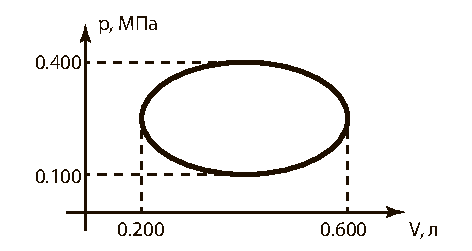
\includegraphics[width=0.5\textwidth]{img01}
\end{wrapfigure}

Количество теплоты получаемое телом за один цикл:
\[
	Q = -A
\]

Работа совершаемая за один цикл можно найти вычислив площадь под графиком:
\[
	A = \pi ab = \pi\frac{p_2 - p_1}{2}\frac{V_2 - V_1}{2}
\]
\[
	A = 3.142\cdot\frac{(0.400-0.100)\cdot10^3}{2}\cdot\frac{0.600-0.200}{2} =
		3.142\cdot0.200\cdot0.150\cdot10^3 \approx 94
\]

Окончательно \( Q = -94 \) Дж.

\newpage
\emph{Задача №2.48}: Первоначально \( 1.00 \) кг азота \((N_2)\) заключен 
в объёме \( V_1 = 0.300 \text{ м}^3 \) под давлением 
\( p_1 = 5.00\cdot10^5 \) Па. Затем газ расширяется, в результате чего 
его объём становится равным \( V_2 = 1.00 \text{ м}^3 \), а давление -- 
равным \( p_2 = 1.00\cdot10^5 \) Па. \\
а) Определить приращение внутренней энергии газа \( \Delta U \). \\
б) Можно ли вычислить работу, совершаемую газом при расширении? \\

\emph{Решение:}

а) Запишем внутренюю энергию идеального газа:

\[
	U = \frac{i}{2}\nu RT, \text{ где i = 5 для } N_2
\]

Найдём приращение внутреней энергии газа:
\begin{equation}
	dU = \frac{i}{2}\nu RdT
	\label{eq:dot}
\end{equation}

Воспользуемся уравнение состояния и найдём \( dT \):
\[
	p_1 V_1 = \nu RT_1, \quad
	p_2 V_2 = \nu RT_2 \Rightarrow
	dT = T_2 - T_1 = \frac{p_2 V_2 - p_1 V_1}{\nu R}
\]

Подставляя последнюю формулу в \label{eq:dot} получаем, с учётом того 
происходит расширение газа, т.е. внутреняя энергия уменьшается:
\[
	dU = -\frac{5}{2}\left( p_1 V_1 - p_2 V_2 \right) = -0.125 \text{ (МДж)}
\]

б) Нет, так как в задаче не указан характер процесса расширения.

\newpage
\emph{Задача №2.78}: Гармонический осциллятор совершает колебания с 
амплитудой \( a \). Масса осциллятора равна m, собственная частота 
\( \omega \). Найти: \\
а) функцию \( f(x) = dP_x/dx \) распределения вероятностей значений 
	координаты \( x \) осциллятора, \\
б) среднее значение координаты \(<x>\), \\
в) среднее значение модуля координаты \(<|x|>\), \\
г) среднее значение квадрата координаты \(<x^2>\), \\
д) среднее значение потенциальной энергии осциллятора \(<U>\). \\

\emph{Решение:}

Используя второй закон Ньютона можно записать уравнение движения для 
гармонического осциллятора в виде:
\[
	m\ddot{x} + kx = 0, \quad
	\ddot{x} + \omega^2 x = 0, \quad \text{ где }\omega^2 = k/m
\]

Решение данного уравнения можно представить в виде:
\[
	x = a\cos(\omega t + \alpha), \quad
	\dot{x} = -a\sin(\omega t + \alpha)
\]

Вероятность найти осциллятор в отрезке \( dx \) можно записать в виде:
\[
	\frac{dP_x}{dx} = \frac{2}{T}\frac{1}{|\dot{x}|}, \quad 
		\text{ где } T = 2\pi/\omega
\]
\[
	dP_x = \frac{2}{T}\frac{dx}{\sin(\omega t + \alpha)} = 
		\frac{dx}{a\pi\sin(\omega t + \alpha)}
\]

Выразим \( \sin(\omega t + \alpha )\) из уравнения движения:
\[
	\frac{x}{a} = \cos(\omega t + \alpha)
\]
\[
	\left( \frac{x}{a} \right)^2 = 1 - \sin^2(\omega t + \alpha) 
		\Rightarrow \sqrt{1-\left( \frac{x}{a} \right)^2} = 
		\sin(\omega t + \alpha)
\]

Подставляя в предыдущую формулу получаем:
\[
	\frac{dP_x}{dx} = \frac{1}{\pi}
		\frac{1}{a\sqrt{1-\left( \frac{x}{a} \right)^2}} = 
		\frac{1}{\pi}\frac{1}{\sqrt{a^2-x^2}}
\]

Проверим нормировку полученной функции:
\[
	\int\limits_{-a}^{a} f(x)dx = 
		\int\limits_{-a}^{a} \frac{1}{\pi}\frac{1}{\sqrt{a^2-x^2}} = 
		\left. 
			\frac{1}{\pi}\arcsin\left( \frac{x}{a} \right) 
		\right|_{-a}^{+a} = \frac{1}{\pi}
		\left( \frac{\pi}{2} + \frac{\pi}{2} \right) = 1
\]

Среднее \( <x> \):
\[
	<x> = \int\limits_{-a}^{+a} xf(x)dx = 
		\int\limits_{-a}^{+a} \frac{xdx}{\sqrt{a^2-x^2}} = 
		\left. -\frac{1}{\pi}\sqrt{a^2-x^2}\right|_{-a}^{+a} = 0 
\]

Найдём среднее \( <|x|> \). Воспользуемся следующими формулами:
\[
	|x|=x\cdot\sign(x), \quad \frac{|x|}{x} = \sign(x)
\]

Тогда интеграл:
\[
	<|x|> = \int\limits_{-a}^{+a} |x|f(x)dx = 
		\sign(x)\int\limits_{-a}^{+a} \frac{xdx}{\sqrt{a^2-x^2}} = 
		\left. 
			-\frac{|x|}{x}\frac{1}{\pi}\sqrt{a^2-x^2} 
		\right|_{-a}^{+a} = 0 
\]

Среднеквадратичное \( <x^2> \):
\[
	<x^2> = \int\limits_{-a}^{+a} x^2f(x)dx =
		\frac{1}{\pi}\int\limits_{-a}^{a} 
		\frac{x^2dx}{\sqrt{a^2-x^2}} = 
		\frac{1}{\pi}\left( x^2\arcsin\frac{x}{a} - 
		\int\limits_{-a}^{+a} 2x \arcsin\frac{x}{a} dx \right)
\]

Делая замену:
\[
	u = x^2, du = 2xdx, dv = \frac{dx}{\sqrt{a^2-x^2}}, 
	v = \arcsin\frac{x}{a}
\]

Окончательно получаем:
\[
	<x^2> = \left. \frac{1}{\pi} \left( 
		\frac{a^2}{2}\arcsin\frac{x}{a} - 
		\frac{x}{2}\sqrt{a^2-x^2} \right)\right|_{-a}^{+a} = 
		\frac{a^2}{2}
\]

Среднее значение потенциально энергии осциллятора, можно записать:
\[
	<U> = \frac{k<x^2>}{2}
\]

Подставляя значения для \( k \) и \( <x^2> \) получаем:
\[
	<U> = \frac{m\omega^2 a^2}{4}
\]

\newpage
\emph{Задача №2.167}: Получить выражение для работы \( A \), совершаемой 
молем ван-дер-ваальсовского газа при изотермическом расширении от объёма 
\( V_1 \) до объёма \( V_2 \). Температура газа \( T \), постоянные 
Ван-дер-Ваальса \( a \) и \( b \). Сравнить полученное выражение с 
аналогичным выражением для идеального газа. \\

\emph{Решение:}

Уравнение состояния газа:
\[
	\left( p + \frac{a}{V^2_m} \right)\left( V_m - b \right) = RT
\]

Для нахождения работы, совершаемой молем ван-дер-ваальсовского газа, 
выразим \( p \) как \( p = p(V_m) \):
\[
	p(V_m) = \frac{RT}{V_m - b} - \frac{a}{V^2_m}
\]

Проинтегрируем выражение от \( V_1 \) до \( V_2 \) и получим \( A \):
\begin{equation}
	A = \int\limits_{V_1}^{V_2} p(V_m) dV_m = 
		\int\limits_{V_1}^{V_2} \left[ 
			\frac{RT}{V_m - b} - \frac{a}{V^2_m}
		\right] dV_m = 
		RT\ln\frac{V_2 - b}{V_1 - b} + a\frac{V_1 - V_2}{V_1 V_2}
	\label{eq:1}
\end{equation}

Для нахождения работы совершаемой идеальным газом, запишем уравнение 
состояния идеального газа в виде:
\[
	pV_m = RT \quad\Rightarrow\quad p(V_m) = \frac{RT}{V_m} 
\]

Совершая аналогичные действия, получаем уравнение для работы в виде:
\begin{equation}
	A = \int\limits_{V_1}^{V_2} p(V_m) dV_m = 
		\int\limits_{V_1}^{V_2} \frac{RT}{V_m} dV_m = 
		RT\ln\frac{V_2}{V_1}
	\label{eq:2}
\end{equation}

Сравнивая уравнение \( \ref{eq:1} \) и \( \ref{eq:2} \) можно увидеть, что 
при устремлении коэффициентов \( a \) и \( b \) к нулю, то уравнение 
\( \ref{eq:1} \) переходит в \( \ref{eq:2} \).

\newpage
\emph{Задача №154}: Моль идеального газа с постоянной теплоёмкостью 
\( C_V \) заключен в цилиндр с адиабатическими стенками и поршнем, который 
может перемещаться в цилиндре без трения. Поршень находится под постоянным 
внешним давлением \( P_1 \). В некоторый момент времени внешнее давление 
скачкообразно уменьшают или увеличивают до \( P_2 \). (Это можно 
достигнуть, снимая часть груза с поршня или добавляя новый груз.) В 
результате газ адиабатически изменяет свой объём. Вычислить температуру и 
объём газа после того, как установится термодинамическое равновесие. \\

\emph{Решение:}

Запишем первое начало термодинамики:
\[
	\delta Q = dU + PdV
\]

Тепло, полученное газом при адиабатическом расширении или сжатии, равно нулю. 
Работа совершаемая газом \( A = P_2 \Delta V \), поэтому 
\( \Delta U + P_2 \Delta V \), с учётом формулы \( U = C_V T \), получаем:
\[
	C_V( T_2 - T ) + P_2 ( V_2 - V_1 ) = 0
\]
\[
	C_V( T_2 - T ) + P_2 V_2 = P_2 V_1
\]

С учётом формулы \( P_2 V_2 = \nu RT_2 \), для одного моля газа, получаем:
\[
	C_V( T_2 - T ) + RT_2 = P_2 V_1
\]

Решая это уравнение относительно \( T_2 \), получаем:
\[
	T_2 = \frac{C_V T + P_2 V_1}{C_V + R} = \frac{C_V T + P_2 V_1}{C_P}
\]

\newpage
\emph{Задача №236}: Доказать соотношения
\[
    \left( \pder{S}{P} \right)_V = 
        \frac{C_V}{T} \left( \pder{T}{P} \right)_V, \quad
    \left( \pder{S}{V} \right)_P = 
        \frac{C_P}{T} \left( \pder{T}{V} \right)_P.
\]

\emph{Решение:}

Используя зависимость энтропии от температуры при постоянном объёме, которое 
выражается через изохорную темлоемкость:
\[
	\frac{C_V}{T} = \left( \pder{S}{T} \right)_V
\]
\[
	\left( \pder{S}{P} \right)_V = \left( \pder{S}{T} \right)_V
		\left( \pder{T}{P} \right)_V = \left( \pder{S}{P} \right)_V
\]

Используя зависимость энтропии от температуры при постоянном давлении, которое 
выражается через изобарную темлоемкость:
\[
	\frac{C_p}{T} = \left( \pder{S}{T} \right)_p
\]
\[
	\left( \pder{S}{V} \right)_p = \left( \pder{S}{T} \right)_p
		\left( \pder{T}{V} \right)_p = \left( \pder{S}{V} \right)_p
\]

Теперь докажем соотношение: 
\[ \left( \pder{S}{T} \right)_V = \frac{C_V}{T} \].

Имеем \( d\Phi = Pdx + Qdy \) формулу для полного дифференциала, где 
\( d\Phi \) -- функция состояния в переменных \( x \) и \( y \), а 
\( P \) и \( Q \) удовлетворяют следующим соотношениям:
\[
	P = \left( \pder{\Phi}{x} \right)_y, \quad
	Q = \left( \pder{\Phi}{y} \right)_x, \quad
	\left( \pder{P}{y} \right)_x = \left( \pder{Q}{x} \right)_y
\] 

Запишем термодинамическое тождество:
\[
	SdT = dU + PdV
\]

Можно заключить, что энтропия \( S = S(T, V) \) является функцией от 
переменных \( T \) и \( V \), тогда её дифференциал равен:
\[
	dS = \frac{dU}{T} + \frac{P}{T}dV \text{ или }
	dS = C_V\frac{dT}{T} + \left( \pder{P}{T} \right)_V dV
\]

Воспользовавщись формулой для полного дифференциала, запишем:
\[
	dS = \left( \pder{S}{T} \right)_V dT + 
		\left( \pder{S}{V} \right)_T dV
\]

Сравнивая формулы заключаем, что:
\[
	\left( \pder{S}{T} \right)_V = \frac{C_V}{T}
\]

Аналогично выводится формула и для второго случая. Имеем формулу: 
\[
	dS = C_p \frac{dT}{T} - \left( \pder{V}{T} \right)_P dP
\]

Сравнивая с
\[
	dS = \left( \pder{S}{T} \right)_P dT + 
		\left( \pder{S}{V} \right)_T dP
\]

Заключаем, что
\[
	\frac{C_P}{T} = \left( \pder{S}{T} \right)_P
\]

\newpage
\emph{Задача №471}: Моль азота расширяется в пустоту от начального объёма 
1 л до конечного 10 л. Найти понижение температуры \( \Delta T \) при 
таком процессе, если постоянная \( a \) в уравнении Ван-дер-Ваальса для 
азота равна \( 1.35\cdot10^6 \text{ атм}\cdot\text{см}^6/\text{моль}^2 \). \\

\emph{Решение:}

Внутреняя энергия ван-дер-ваальсовского газа \( U = K + U_1 \), где 
\( K \) -- суммарная кинетическая энергия молекул, а \( U_1 \) -- суммарная 
энергия взаимодействия молекул. Работа сил притяжения равна убыли энергии 
\( U_1 \) : \( dA = -dU_1 \). Силы притяжения характеризуются внутренним 
давлением \( p_i = a / V^2_m \). Тогда элементарная работа этих сил
\( d'A = -p_i dV_m \), где знак минус обусловлен тем, что при расширении газа 
работа \( d'A < 0 \).
\[
	d'A = -\frac{a}{V^2_m} = -d\left( -\frac{a}{V_m} \right), \quad
	U_1 = -\frac{a}{V_m}
\] 

Суммарная кинетическая энергия \( K \) зависит от поступательного и 
внутреннего движения молекул, и определяется как \( C_V T \). Таким образом 
получаем уравнение:
\begin{equation}
	U_m = C_V T - \frac{a}{V_m}
	\label{eq:3}
\end{equation} 

Так как газ расширяется в пустоту без теплообмена, то \( A = 0, Q = 0 \), и 
согласно первому началу \( U = const \).

Согласно уравнению \( \ref{eq:3} \) и \( U = const \):
\[
	\Delta U = \nu C_V \Delta T - \nu^2 a 
		\left( \frac{1}{V_2} - \frac{1}{V_1} \right) = 0
\]

Окончательно получаем:
\[
	\Delta T = \nu\frac{a}{C_V}\left( \frac{1}{V_1} - \frac{1}{V_2} \right) = 
		0.25 \text{ } (^\circ C)
\]

\end{document}
